%!TEX root = Main.tex

\section{Simulation}

We analyze the network with two types of nodes.
The first type of nodes (type I) are equispaced points on $x=1$ and $0\leq y\leq 6$.
The second type of nodes (type II) are generated uniformly in $[0,2]\times[0,6]$. 
Figure \ref{fig: nodes} gives an example of 30 nodes, among which 3 are from type I and the rest 27 are from type II.
\\
\begin{figure}[H]
\centering
\includegraphics[width=0.5\textwidth]{../simulation/nodes_distribution}
\caption{30 nodes with three belonging to group 1.}
\label{fig: nodes}
\end{figure}

Some edges are constructed between pairs of nodes during time period $[0,50]$.
Nodes are connected if and only if there distance is less than $1.5$.
For the nodes of the same type, the connecting time is generated from uniform distribution $U(0,40)$.
For the pair of nodes with one from type I and the other from type II, the connecting time is distributed as $N(5+\tau,1)$, where $\tau$ is the time delay caused by the type I node and is generated randomly from $U(0,30)$.

The case with 3 type I nodes and 27 type II nodes is tested.
Clustering error rate is recorded for 10 independent trials. 
Due to the uncertainty caused by initialization, five independent initializations are used for each trial, and only the one with the largest distance between estimated mean curves is kept.
The average error rate is $1.3/30=4.3\%$.



% To show the development of the network, we plot snapshots in Fig.\ref{Fig: development of network} of the network $\mathbf{G}_1$  at time points $t=0.01, 0.1, 1, 10, 100$.
% \begin{figure}
% \centering
% 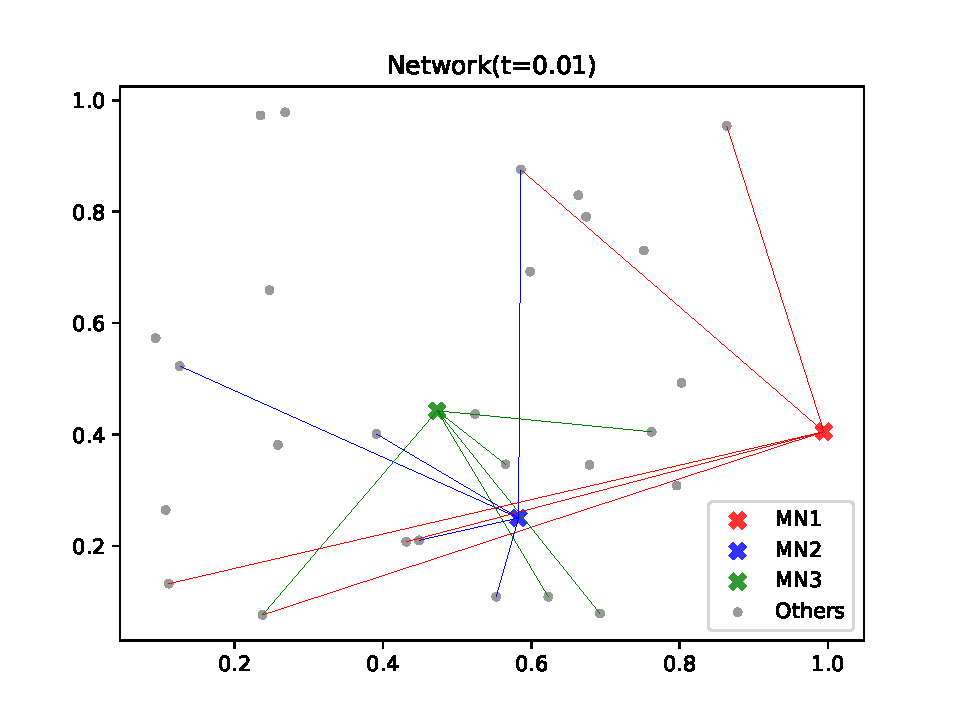
\includegraphics[width = 0.3\textwidth]{Graphs/t_001.pdf}
% 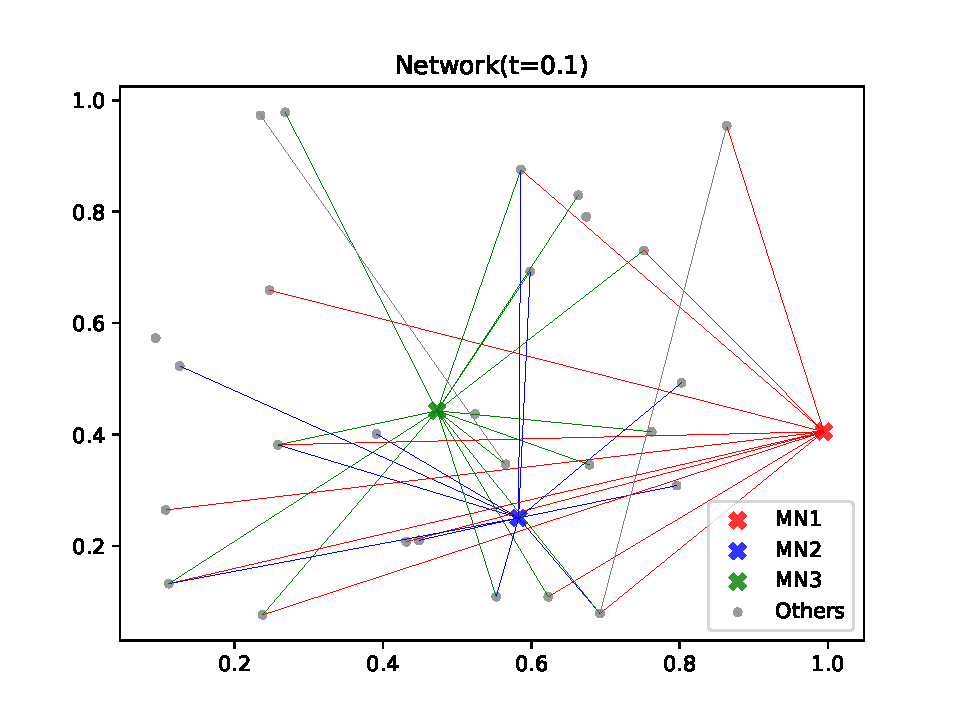
\includegraphics[width = 0.3\textwidth]{Graphs/t_01.pdf}
% 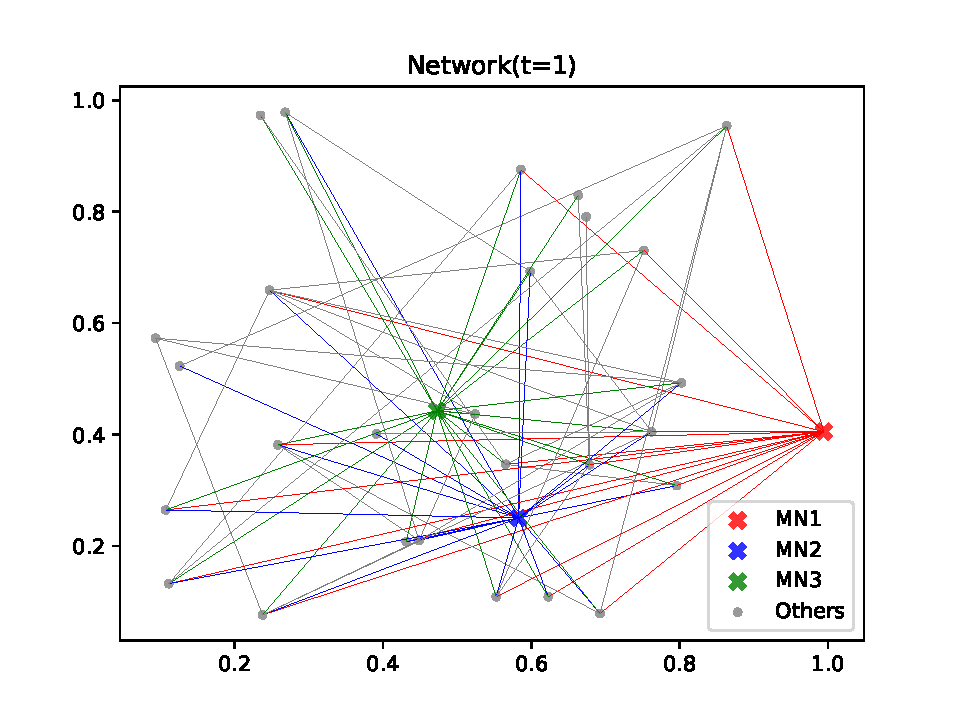
\includegraphics[width = 0.3\textwidth]{Graphs/t_1.pdf}\\
% 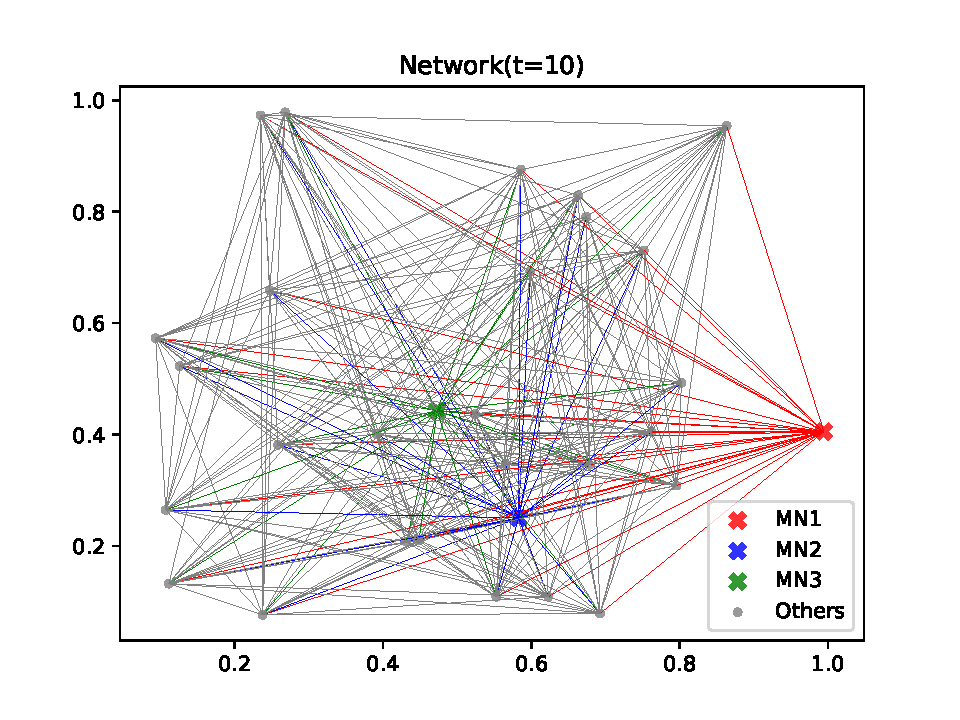
\includegraphics[width = 0.3\textwidth]{Graphs/t_10.pdf}
% 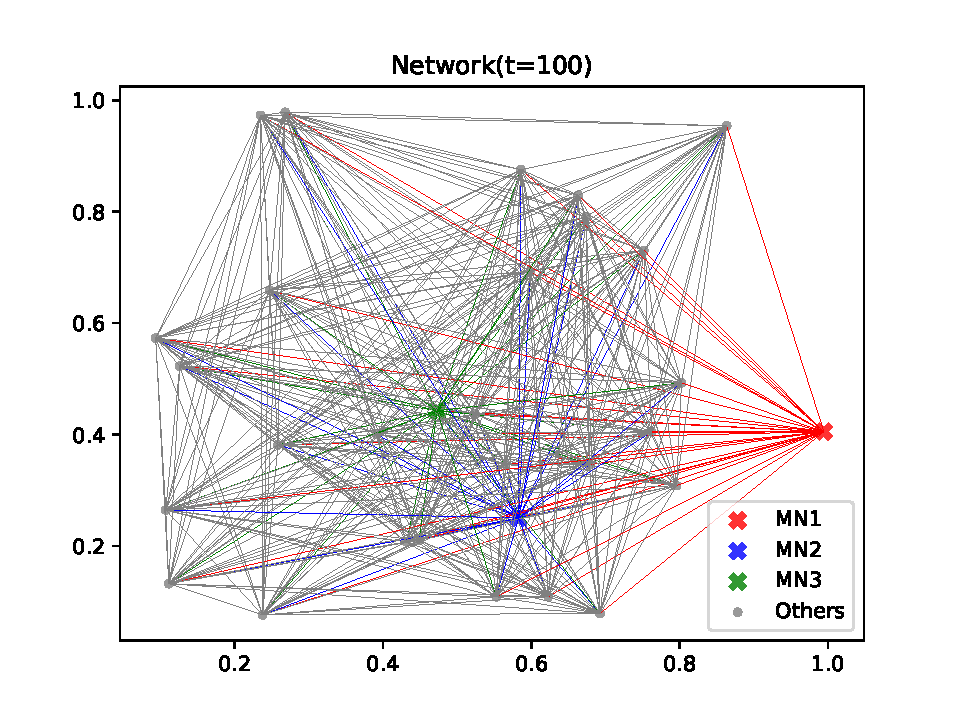
\includegraphics[width = 0.3\textwidth]{Graphs/t_100.pdf}
% \caption{Development of the network with two cell types. The node $n_1$ is represented by ``MN1'' in red. The node $n_2$ is represented by ``MN2'' in blue. The node $n_3$ is represented by ``MN3'' in green. Other nodes are represented by ``Others'' in gray.}
% \label{Fig: development of network}
% \end{figure}


